Nous avons développé une interface web complète montrant les possibilités qu’une smartcity comme la nôtre peut apporter. Cette interface nous permet non seulement de manager la ville dans son ensemble, mais aussi de visualiser l’état de chaque capteur, ainsi que l’historique des données. Nous avons tenté ici de démontrer la facilité avec laquelle notre infrastructure permet d’être utilisée dans une optique big data. Ainsi, bien que notre interface soit simple, nous constatons que la multitude de données fournies par notre API peut être agrégée et traitée afin d’en retirer des informations plus pertinentes.

\subsection{Dashboard}
\begin{figure}[H]
    \begin{center}
        \frame{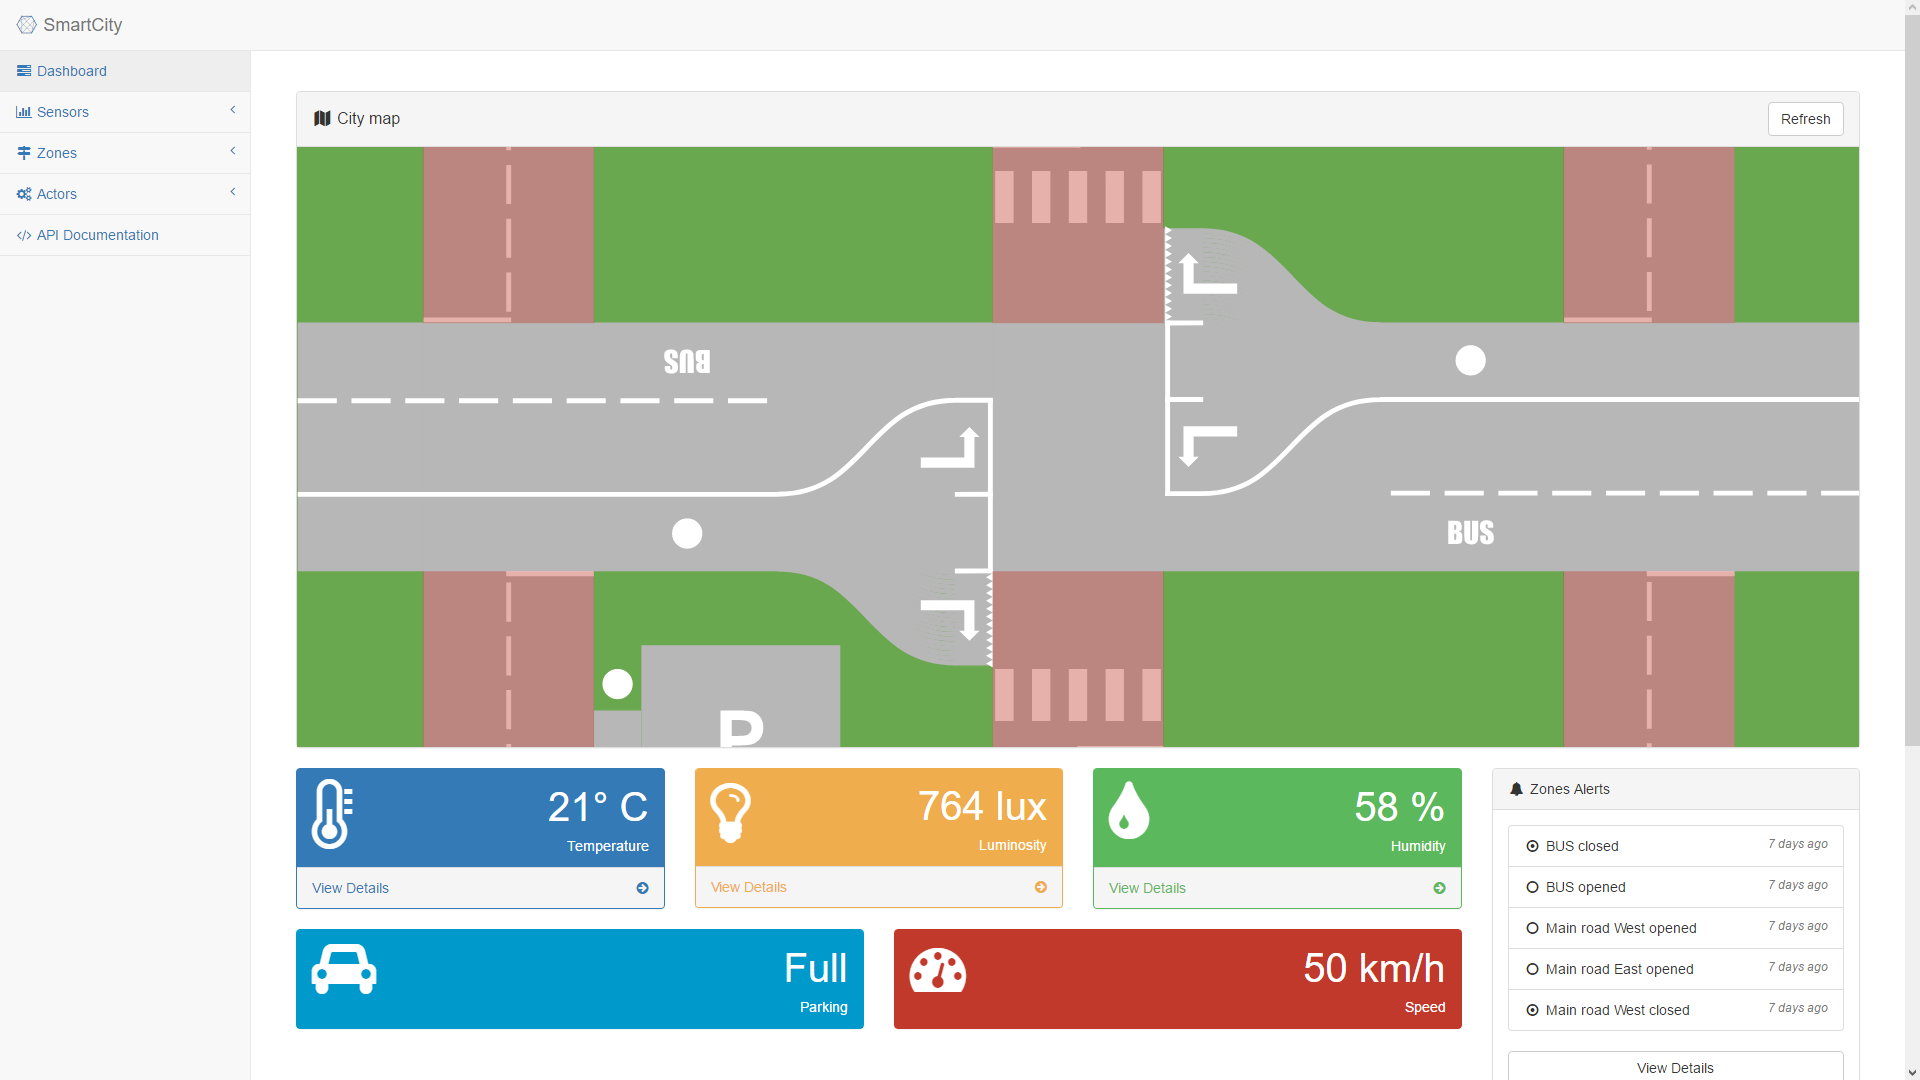
\includegraphics[width=\linewidth, height=\textheight,keepaspectratio]{img/dashboard}}

        \caption{Dashboard} \label{dashboard}
    \end{center}
\end{figure}
L’illustration (\ref{dashboard}) ci-dessus représente le dashboard de notre interface web. Il permet de visualiser les données importantes fournies par divers capteurs sur la maquette (température, luminosité …). De plus la carte interactive, permettant les mêmes "gestuelles" que sur des services tel que Google Maps (zoom, mouvement grâce au pointeur, etc.), est la représentation en temps réel de notre ville. Ainsi, si nous souhaitons connaître l’état d’un capteur, il suffit de placer sa souris à l’endroit voulu pour obtenir l’information (illustration \ref{etat-capteur}).
\begin{figure}[H]
    \begin{center}
        \frame{
        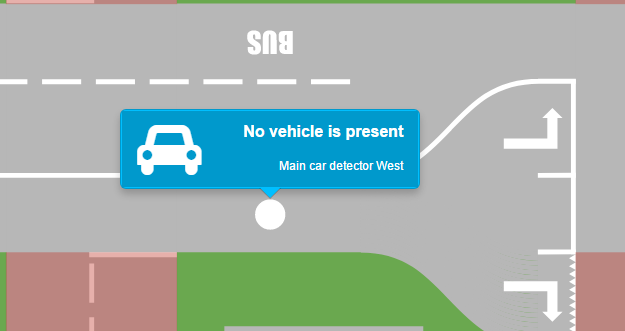
\includegraphics[scale=0.4,keepaspectratio]{img/detail_capteur_map}}
        \caption{Affichage de l'état d'un capteur sur la carte}\label{etat-capteur}
    \end{center}
\end{figure}
\vspace{-0.5cm}
Sur cet écran d’accueil, nous pouvons aussi visualiser un court historique concernant les ouvertures/fermetures des différentes zones ainsi qu’un historique des accès au parking de notre ville.

\subsection{Sensors}
La rubrique senseurs reprend quant à elle l’historique des principaux senseurs. Comme le montre l’illustration ci-dessous (\ref{senseurs}), nous avons représenté les informations sous forme de graphe. Nous pouvons appliquer des filtres afin d’afficher les données de la dernière heure, du dernier mois ou de la dernière année et aussi choisir le nombre de périodes (heure, mois et année). Tous ces graphes utilisent notre API afin de récupérer les données fournies par notre ville intelligente.
\begin{figure}[H]
    \begin{center}
        \frame{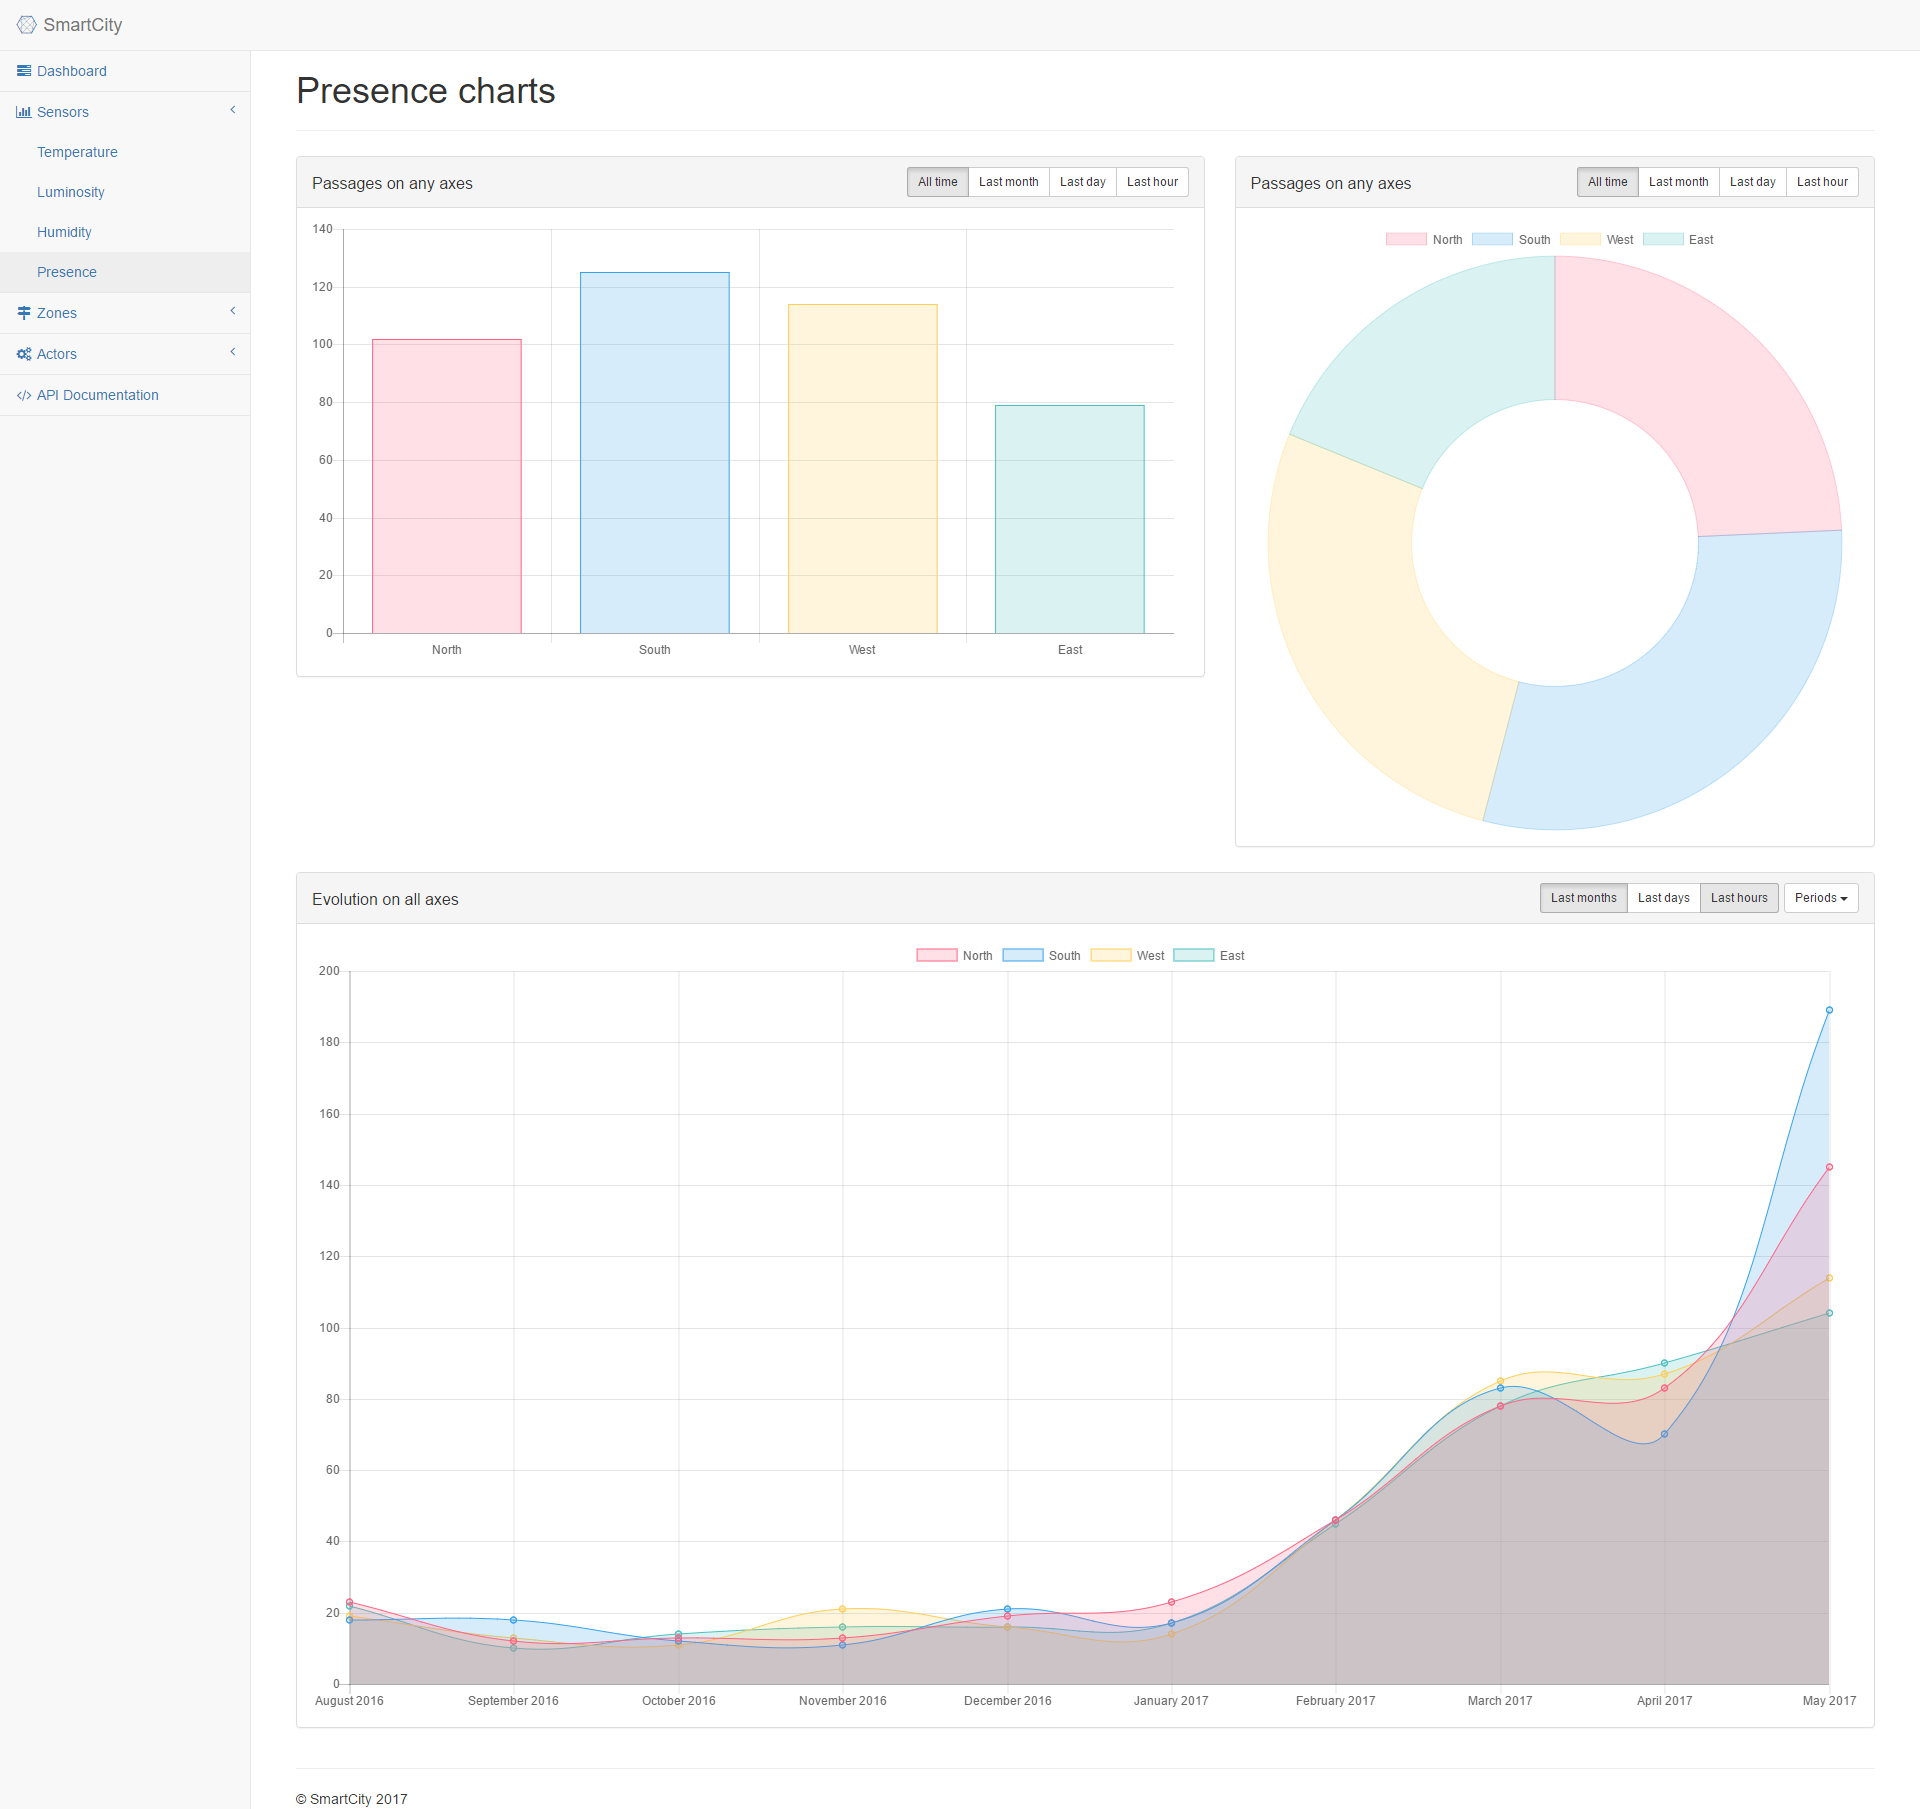
\includegraphics[width=\linewidth, height=\textheight,keepaspectratio]{img/interface_senseurs}}
        \caption{Historique des capteurs de présence sur les 4 axes routier}\label{senseurs}
    \end{center}
\end{figure}

\subsection{Zones}
Cette rubrique (illustration \ref{senseurs}) permet la gestion des zones de notre ville. Ainsi, nous pouvons ouvrir/fermer des zones ou ajouter/supprimer des horaires de bus afin de gérer dynamiquement les heures d’ouverture de la zone bus.
\begin{figure}[H]
    \begin{center}
        \frame{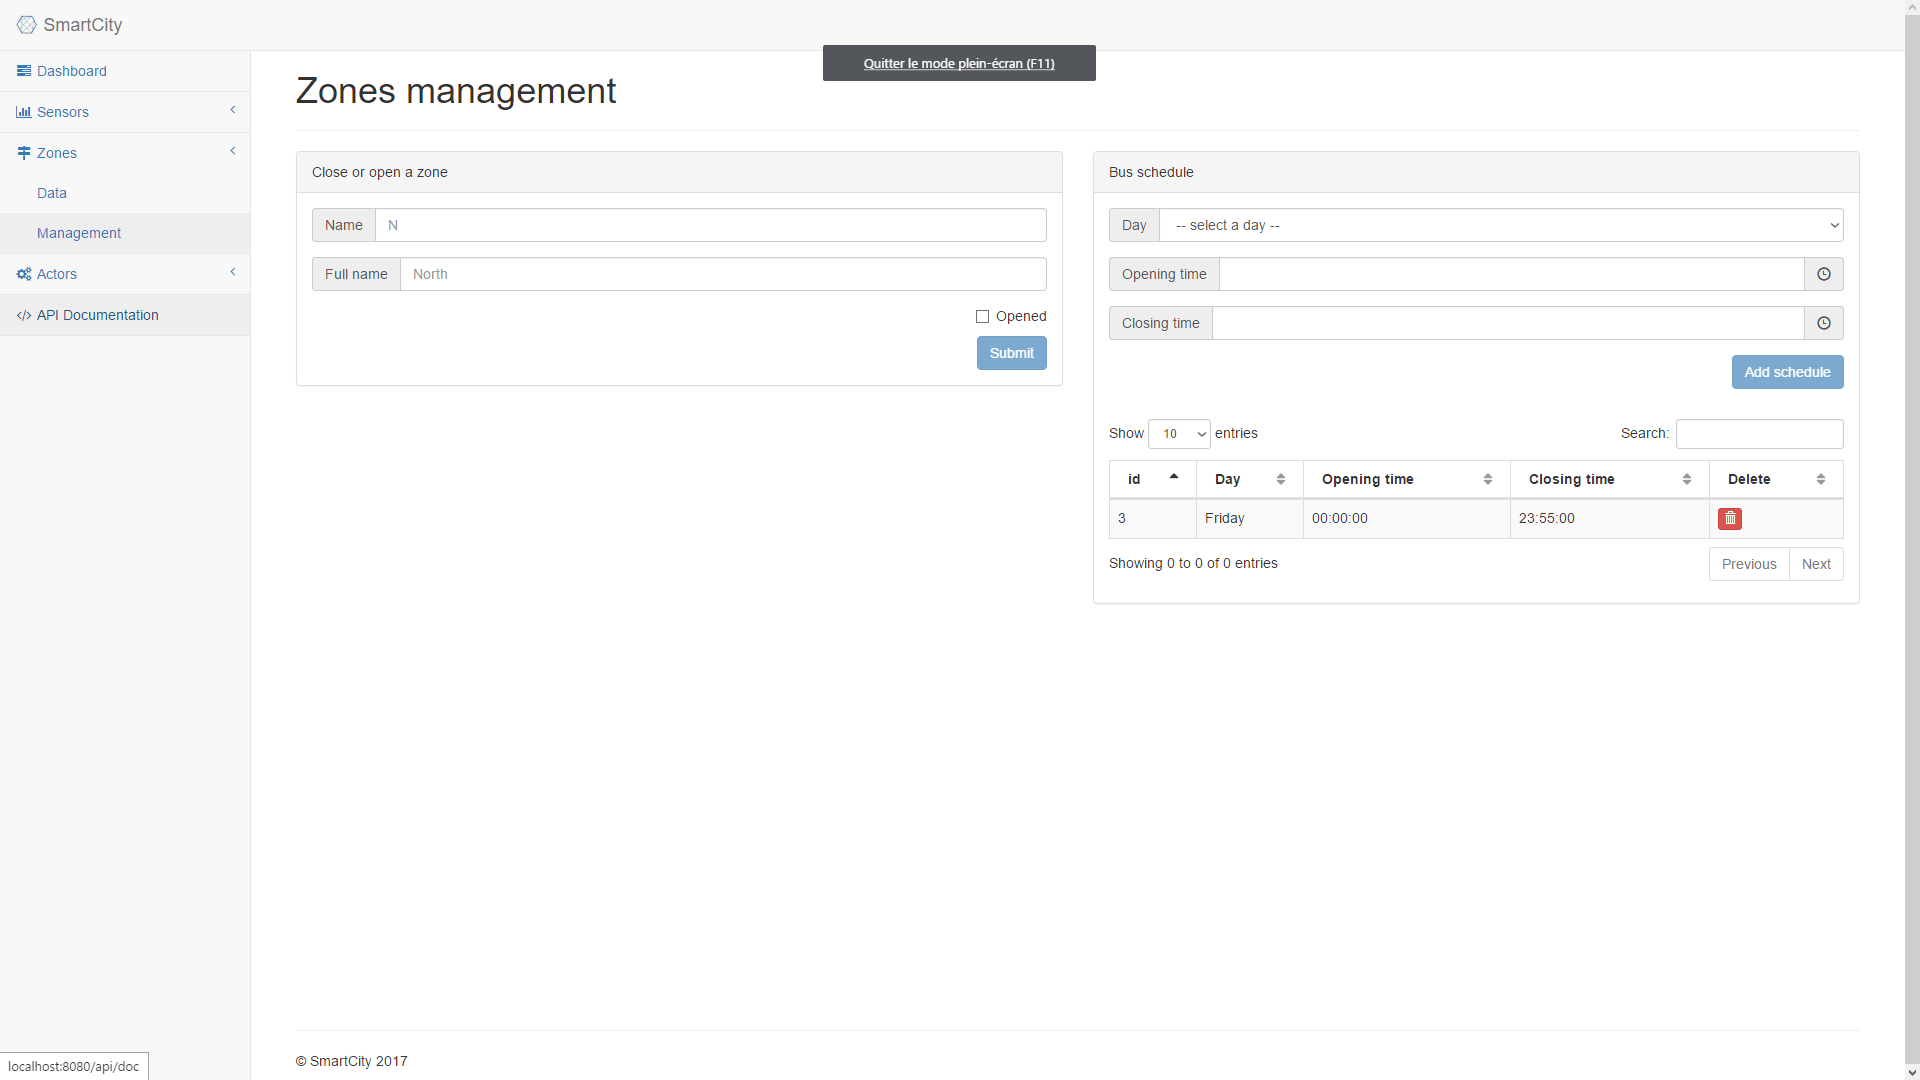
\includegraphics[width=\linewidth, height=\textheight,keepaspectratio]{img/interface_zones}}
        \caption{Interface pour contrôler les zones}\label{senseurs}
    \end{center}
\end{figure}

\subsection{Actor}
Cette rubrique permet de lancer ou de stopper notre ville intelligente. Cette fonctionnalité n’est pas vouée à être présente dans une version de production, mais nous permet de facilement démarrer/arrêter notre ville pendant la phase de test afin de montrer la facilité qu’a notre système à redémarrer.

\subsection{API Documentation}
À nouveau, cette partie du site n’est pas vouée à être disponible pour le grand public, mais bien à un public de développeurs. C’est le point d’entrée pour permettre à des services externes d’utiliser les données de notre ville. Nous offrons ainsi une vision open data de notre ville intelligente. À noter que nous utilisons Swagger afin de générer la documentation de notre API (illustration \ref{doc}).
\begin{figure}[H]
    \begin{center}
        \frame{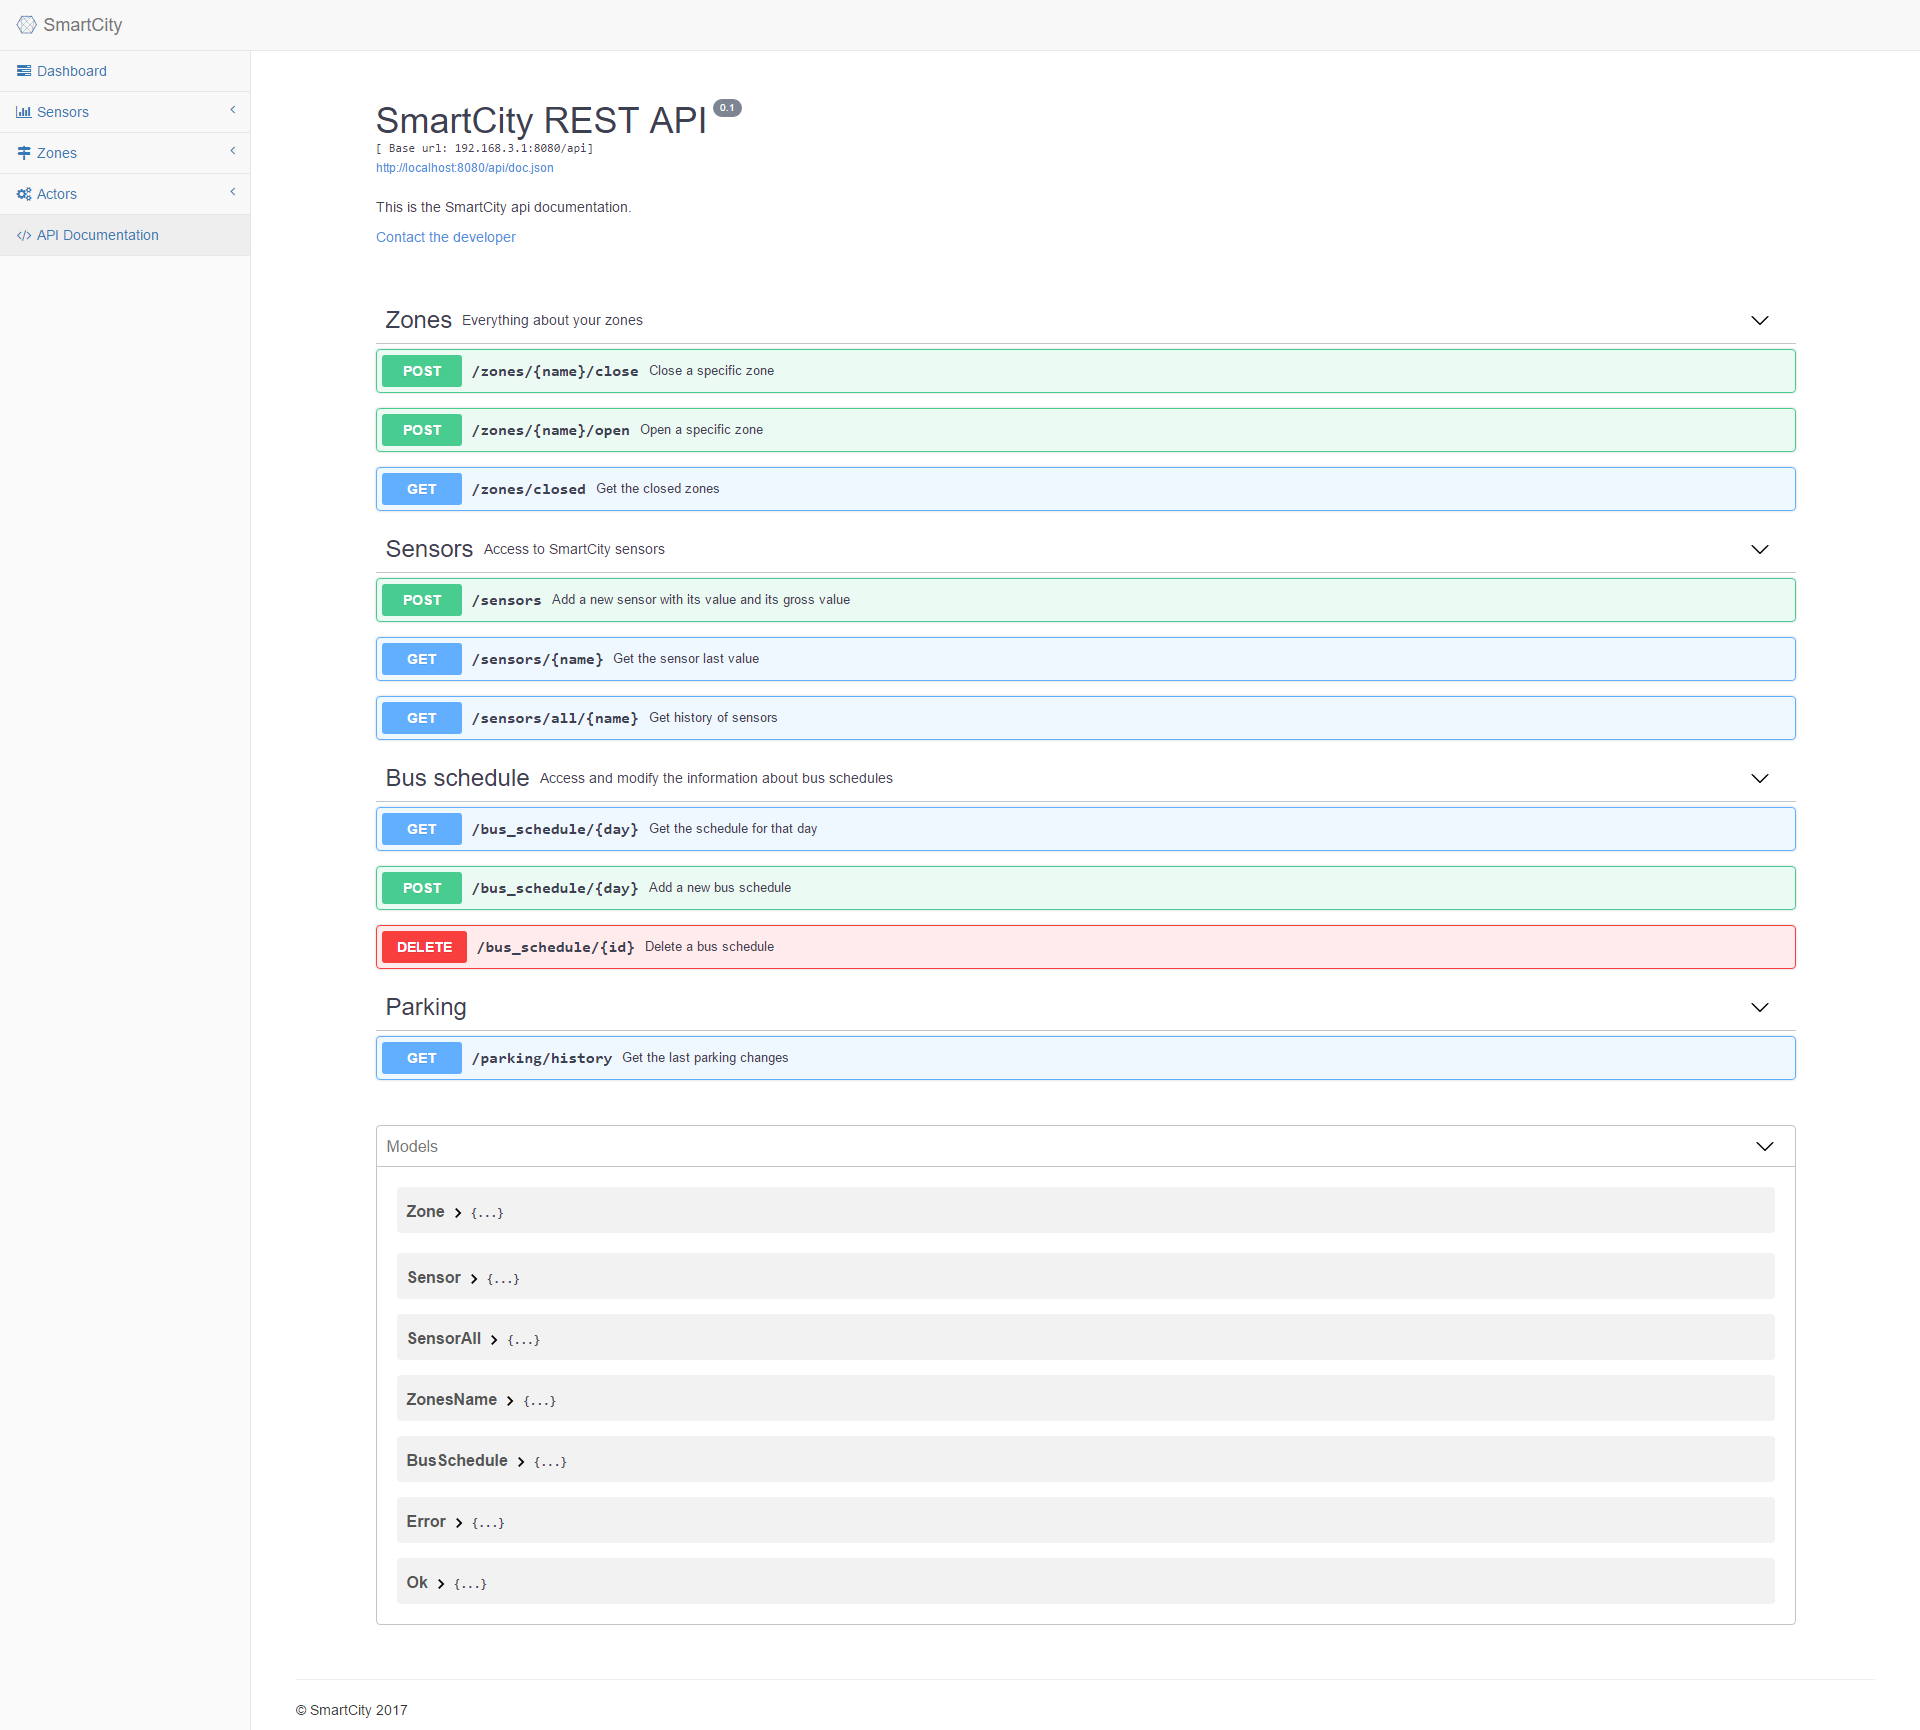
\includegraphics[width=\linewidth, height=\textheight,keepaspectratio]{img/interface_API}}
        \caption{Interface documentant notre API}\label{doc}
    \end{center}
\end{figure}